\documentclass[]{article}
\usepackage{lmodern}
\usepackage{amssymb,amsmath}
\usepackage{ifxetex,ifluatex}
\usepackage{fixltx2e} % provides \textsubscript
\ifnum 0\ifxetex 1\fi\ifluatex 1\fi=0 % if pdftex
  \usepackage[T1]{fontenc}
  \usepackage[utf8]{inputenc}
\else % if luatex or xelatex
  \ifxetex
    \usepackage{mathspec}
  \else
    \usepackage{fontspec}
  \fi
  \defaultfontfeatures{Ligatures=TeX,Scale=MatchLowercase}
\fi
% use upquote if available, for straight quotes in verbatim environments
\IfFileExists{upquote.sty}{\usepackage{upquote}}{}
% use microtype if available
\IfFileExists{microtype.sty}{%
\usepackage{microtype}
\UseMicrotypeSet[protrusion]{basicmath} % disable protrusion for tt fonts
}{}
\usepackage[margin=1in]{geometry}
\usepackage{hyperref}
\hypersetup{unicode=true,
            pdftitle={Final Project},
            pdfborder={0 0 0},
            breaklinks=true}
\urlstyle{same}  % don't use monospace font for urls
\usepackage{color}
\usepackage{fancyvrb}
\newcommand{\VerbBar}{|}
\newcommand{\VERB}{\Verb[commandchars=\\\{\}]}
\DefineVerbatimEnvironment{Highlighting}{Verbatim}{commandchars=\\\{\}}
% Add ',fontsize=\small' for more characters per line
\usepackage{framed}
\definecolor{shadecolor}{RGB}{248,248,248}
\newenvironment{Shaded}{\begin{snugshade}}{\end{snugshade}}
\newcommand{\KeywordTok}[1]{\textcolor[rgb]{0.13,0.29,0.53}{\textbf{#1}}}
\newcommand{\DataTypeTok}[1]{\textcolor[rgb]{0.13,0.29,0.53}{#1}}
\newcommand{\DecValTok}[1]{\textcolor[rgb]{0.00,0.00,0.81}{#1}}
\newcommand{\BaseNTok}[1]{\textcolor[rgb]{0.00,0.00,0.81}{#1}}
\newcommand{\FloatTok}[1]{\textcolor[rgb]{0.00,0.00,0.81}{#1}}
\newcommand{\ConstantTok}[1]{\textcolor[rgb]{0.00,0.00,0.00}{#1}}
\newcommand{\CharTok}[1]{\textcolor[rgb]{0.31,0.60,0.02}{#1}}
\newcommand{\SpecialCharTok}[1]{\textcolor[rgb]{0.00,0.00,0.00}{#1}}
\newcommand{\StringTok}[1]{\textcolor[rgb]{0.31,0.60,0.02}{#1}}
\newcommand{\VerbatimStringTok}[1]{\textcolor[rgb]{0.31,0.60,0.02}{#1}}
\newcommand{\SpecialStringTok}[1]{\textcolor[rgb]{0.31,0.60,0.02}{#1}}
\newcommand{\ImportTok}[1]{#1}
\newcommand{\CommentTok}[1]{\textcolor[rgb]{0.56,0.35,0.01}{\textit{#1}}}
\newcommand{\DocumentationTok}[1]{\textcolor[rgb]{0.56,0.35,0.01}{\textbf{\textit{#1}}}}
\newcommand{\AnnotationTok}[1]{\textcolor[rgb]{0.56,0.35,0.01}{\textbf{\textit{#1}}}}
\newcommand{\CommentVarTok}[1]{\textcolor[rgb]{0.56,0.35,0.01}{\textbf{\textit{#1}}}}
\newcommand{\OtherTok}[1]{\textcolor[rgb]{0.56,0.35,0.01}{#1}}
\newcommand{\FunctionTok}[1]{\textcolor[rgb]{0.00,0.00,0.00}{#1}}
\newcommand{\VariableTok}[1]{\textcolor[rgb]{0.00,0.00,0.00}{#1}}
\newcommand{\ControlFlowTok}[1]{\textcolor[rgb]{0.13,0.29,0.53}{\textbf{#1}}}
\newcommand{\OperatorTok}[1]{\textcolor[rgb]{0.81,0.36,0.00}{\textbf{#1}}}
\newcommand{\BuiltInTok}[1]{#1}
\newcommand{\ExtensionTok}[1]{#1}
\newcommand{\PreprocessorTok}[1]{\textcolor[rgb]{0.56,0.35,0.01}{\textit{#1}}}
\newcommand{\AttributeTok}[1]{\textcolor[rgb]{0.77,0.63,0.00}{#1}}
\newcommand{\RegionMarkerTok}[1]{#1}
\newcommand{\InformationTok}[1]{\textcolor[rgb]{0.56,0.35,0.01}{\textbf{\textit{#1}}}}
\newcommand{\WarningTok}[1]{\textcolor[rgb]{0.56,0.35,0.01}{\textbf{\textit{#1}}}}
\newcommand{\AlertTok}[1]{\textcolor[rgb]{0.94,0.16,0.16}{#1}}
\newcommand{\ErrorTok}[1]{\textcolor[rgb]{0.64,0.00,0.00}{\textbf{#1}}}
\newcommand{\NormalTok}[1]{#1}
\usepackage{graphicx,grffile}
\makeatletter
\def\maxwidth{\ifdim\Gin@nat@width>\linewidth\linewidth\else\Gin@nat@width\fi}
\def\maxheight{\ifdim\Gin@nat@height>\textheight\textheight\else\Gin@nat@height\fi}
\makeatother
% Scale images if necessary, so that they will not overflow the page
% margins by default, and it is still possible to overwrite the defaults
% using explicit options in \includegraphics[width, height, ...]{}
\setkeys{Gin}{width=\maxwidth,height=\maxheight,keepaspectratio}
\IfFileExists{parskip.sty}{%
\usepackage{parskip}
}{% else
\setlength{\parindent}{0pt}
\setlength{\parskip}{6pt plus 2pt minus 1pt}
}
\setlength{\emergencystretch}{3em}  % prevent overfull lines
\providecommand{\tightlist}{%
  \setlength{\itemsep}{0pt}\setlength{\parskip}{0pt}}
\setcounter{secnumdepth}{0}
% Redefines (sub)paragraphs to behave more like sections
\ifx\paragraph\undefined\else
\let\oldparagraph\paragraph
\renewcommand{\paragraph}[1]{\oldparagraph{#1}\mbox{}}
\fi
\ifx\subparagraph\undefined\else
\let\oldsubparagraph\subparagraph
\renewcommand{\subparagraph}[1]{\oldsubparagraph{#1}\mbox{}}
\fi

%%% Use protect on footnotes to avoid problems with footnotes in titles
\let\rmarkdownfootnote\footnote%
\def\footnote{\protect\rmarkdownfootnote}

%%% Change title format to be more compact
\usepackage{titling}

% Create subtitle command for use in maketitle
\newcommand{\subtitle}[1]{
  \posttitle{
    \begin{center}\large#1\end{center}
    }
}

\setlength{\droptitle}{-2em}

  \title{Final Project}
    \pretitle{\vspace{\droptitle}\centering\huge}
  \posttitle{\par}
    \author{}
    \preauthor{}\postauthor{}
    \date{}
    \predate{}\postdate{}
  

\begin{document}
\maketitle

\subsection{R Markdown}\label{r-markdown}

\begin{Shaded}
\begin{Highlighting}[]
\CommentTok{# install.packages("arules")}

\KeywordTok{library}\NormalTok{(arules)}
\end{Highlighting}
\end{Shaded}

\begin{verbatim}
## Loading required package: Matrix
\end{verbatim}

\begin{verbatim}
## 
## Attaching package: 'arules'
\end{verbatim}

\begin{verbatim}
## The following objects are masked from 'package:base':
## 
##     abbreviate, write
\end{verbatim}

\begin{Shaded}
\begin{Highlighting}[]
\NormalTok{data <-}\StringTok{ }\KeywordTok{read.csv}\NormalTok{(}\DataTypeTok{file =} \StringTok{"AppleStoreClean.csv"}\NormalTok{, }\DataTypeTok{head =} \OtherTok{TRUE}\NormalTok{)}
\NormalTok{tdata <-}\StringTok{ }\KeywordTok{read.transactions}\NormalTok{(}\StringTok{"AppleStoreClean.csv"}\NormalTok{, }\DataTypeTok{quote=}\StringTok{""}\NormalTok{, }\DataTypeTok{sep=}\StringTok{","}\NormalTok{)}
\end{Highlighting}
\end{Shaded}

\begin{verbatim}
## Warning in asMethod(object): removing duplicated items in transactions
\end{verbatim}

\subsection{HCLUST}\label{hclust}

\begin{Shaded}
\begin{Highlighting}[]
\NormalTok{distance =}\StringTok{ }\KeywordTok{dist}\NormalTok{(}\KeywordTok{as.matrix}\NormalTok{(data), }\DataTypeTok{method =} \StringTok{"euclidean"}\NormalTok{)}
\end{Highlighting}
\end{Shaded}

\begin{verbatim}
## Warning in dist(as.matrix(data), method = "euclidean"): NAs introduced by
## coercion
\end{verbatim}

\begin{Shaded}
\begin{Highlighting}[]
\CommentTok{# perform clustering}
\NormalTok{hc =}\StringTok{ }\KeywordTok{hclust}\NormalTok{(distance)}

\CommentTok{# cut the tree}
\NormalTok{clusterCut <-}\StringTok{ }\KeywordTok{cutree}\NormalTok{(hc, }\DecValTok{300}\NormalTok{)}

\CommentTok{# plot dendrogram}
\KeywordTok{plot}\NormalTok{(clusterCut)}
\end{Highlighting}
\end{Shaded}

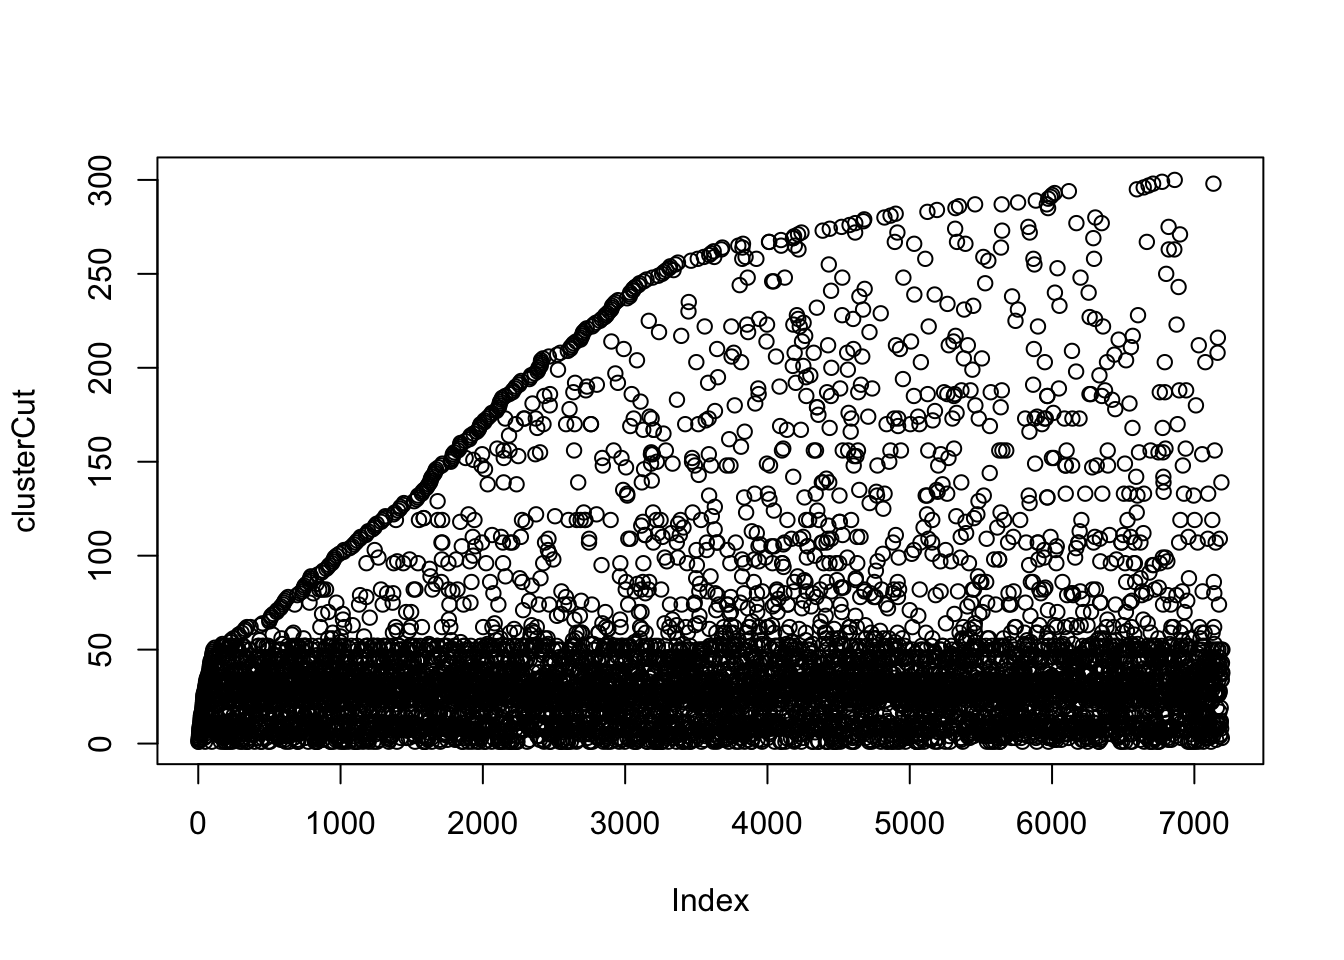
\includegraphics{final_project_files/figure-latex/unnamed-chunk-2-1.pdf}

\begin{Shaded}
\begin{Highlighting}[]
\CommentTok{#write.csv(clusterCut, file = "C:\textbackslash{}\textbackslash{}Users\textbackslash{}\textbackslash{}samue\textbackslash{}\textbackslash{}Desktop\textbackslash{}\textbackslash{}hclust.csv")}
\end{Highlighting}
\end{Shaded}

\subsection{Apriori}\label{apriori}

\begin{Shaded}
\begin{Highlighting}[]
\NormalTok{apprules <-}\StringTok{ }\KeywordTok{apriori}\NormalTok{(tdata, }\DataTypeTok{parameter =} \KeywordTok{list}\NormalTok{(}\DataTypeTok{support =} \FloatTok{0.01}\NormalTok{, }\DataTypeTok{confidence =} \FloatTok{0.35}\NormalTok{, }\DataTypeTok{minlen =} \DecValTok{2}\NormalTok{))}
\end{Highlighting}
\end{Shaded}

\begin{verbatim}
## Apriori
## 
## Parameter specification:
##  confidence minval smax arem  aval originalSupport maxtime support minlen
##        0.35    0.1    1 none FALSE            TRUE       5    0.01      2
##  maxlen target   ext
##      10  rules FALSE
## 
## Algorithmic control:
##  filter tree heap memopt load sort verbose
##     0.1 TRUE TRUE  FALSE TRUE    2    TRUE
## 
## Absolute minimum support count: 71 
## 
## set item appearances ...[0 item(s)] done [0.00s].
## set transactions ...[18421 item(s), 7198 transaction(s)] done [0.03s].
## sorting and recoding items ... [67 item(s)] done [0.00s].
## creating transaction tree ... done [0.00s].
## checking subsets of size 1 2 3 4 5 6 7 done [0.01s].
## writing ... [4520 rule(s)] done [0.00s].
## creating S4 object  ... done [0.01s].
\end{verbatim}

\begin{Shaded}
\begin{Highlighting}[]
\KeywordTok{summary}\NormalTok{(apprules)}
\end{Highlighting}
\end{Shaded}

\begin{verbatim}
## set of 4520 rules
## 
## rule length distribution (lhs + rhs):sizes
##    2    3    4    5    6    7 
##  313 1318 1669  937  262   21 
## 
##    Min. 1st Qu.  Median    Mean 3rd Qu.    Max. 
##   2.000   3.000   4.000   3.907   5.000   7.000 
## 
## summary of quality measures:
##     support          confidence          lift            count       
##  Min.   :0.01000   Min.   :0.3502   Min.   :0.5062   Min.   :  72.0  
##  1st Qu.:0.01292   1st Qu.:0.4876   1st Qu.:0.9149   1st Qu.:  93.0  
##  Median :0.01848   Median :0.5953   Median :1.0263   Median : 133.0  
##  Mean   :0.03435   Mean   :0.5999   Mean   :1.0682   Mean   : 247.2  
##  3rd Qu.:0.03418   3rd Qu.:0.6949   3rd Qu.:1.1626   3rd Qu.: 246.0  
##  Max.   :0.43137   Max.   :1.0000   Max.   :5.9464   Max.   :3105.0  
## 
## mining info:
##   data ntransactions support confidence
##  tdata          7198    0.01       0.35
\end{verbatim}

\begin{Shaded}
\begin{Highlighting}[]
\KeywordTok{inspect}\NormalTok{(}\KeywordTok{sort}\NormalTok{(apprules, }\DataTypeTok{by =} \StringTok{"confidence"}\NormalTok{)[}\DecValTok{1}\OperatorTok{:}\DecValTok{20}\NormalTok{])}
\end{Highlighting}
\end{Shaded}

\begin{verbatim}
##      lhs                     rhs       support    confidence lift    
## [1]  {"Shopping"}         => {0}       0.01694915 1.0000000  1.468081
## [2]  {"Shopping",37}      => {0}       0.01389275 1.0000000  1.468081
## [3]  {"4+","Shopping"}    => {0}       0.01139205 1.0000000  1.468081
## [4]  {"9+",6.99}          => {"Games"} 0.01500417 1.0000000  1.863801
## [5]  {"Education",3}      => {"4+"}    0.01000278 1.0000000  1.623731
## [6]  {"4+","Shopping",37} => {0}       0.01014171 1.0000000  1.468081
## [7]  {"9+",5,6.99}        => {"Games"} 0.01472631 1.0000000  1.863801
## [8]  {"9+",0,40,5}        => {"Games"} 0.01055849 1.0000000  1.863801
## [9]  {"9+",40,5}          => {"Games"} 0.01986663 0.9930556  1.850858
## [10] {"Education",3.5}    => {"4+"}    0.01403168 0.9901961  1.607812
## [11] {"9+",1,40,5}        => {"Games"} 0.01375382 0.9900000  1.845163
## [12] {"Education",3.5,5}  => {"4+"}    0.01236455 0.9888889  1.605690
## [13] {"Education",40}     => {"4+"}    0.01208669 0.9886364  1.605280
## [14] {"Education",4}      => {"4+"}    0.02389553 0.9885057  1.605068
## [15] {"9+",43,5}          => {"Games"} 0.01097527 0.9875000  1.840504
## [16] {"9+",0,38,4.5,5}    => {"Games"} 0.01097527 0.9875000  1.840504
## [17] {"9+",24}            => {5}       0.01055849 0.9870130  1.421472
## [18] {"9+","Games",24}    => {5}       0.01028063 0.9866667  1.420974
## [19] {"Education",2.99}   => {"4+"}    0.02042234 0.9865772  1.601936
## [20] {"Education",40,5}   => {"4+"}    0.01014171 0.9864865  1.601789
##      count
## [1]  122  
## [2]  100  
## [3]   82  
## [4]  108  
## [5]   72  
## [6]   73  
## [7]  106  
## [8]   76  
## [9]  143  
## [10] 101  
## [11]  99  
## [12]  89  
## [13]  87  
## [14] 172  
## [15]  79  
## [16]  79  
## [17]  76  
## [18]  74  
## [19] 147  
## [20]  73
\end{verbatim}

\begin{Shaded}
\begin{Highlighting}[]
\CommentTok{#itemFrequencyPlot(tdata, support = 0.1) # items with a support of 0.1}
\CommentTok{#itemFrequencyPlot(tdata, topN = 20) # 20 most frequent items}
\end{Highlighting}
\end{Shaded}

\subsection{K-Means}\label{k-means}

\subsection{Cut the tree}\label{cut-the-tree}

\begin{Shaded}
\begin{Highlighting}[]
\CommentTok{#clusterCut <- cutree(hc, 10)}
\CommentTok{#library(cluster)}
\CommentTok{#clusplot(clusterCut, color=TRUE, shade=TRUE, labels=2, lines=0)}
\end{Highlighting}
\end{Shaded}


\end{document}
